\section{Application}
\label{sec:takeaways}
We apply our proposed formulation to validate and provide a theoretical explanation for numerous existing experimental findings regarding the training dynamics of language models. These key insights also guide researchers in selecting critical LRS before initiating model training. An interesting summary is that
\begin{quotation}
{\color{magenta}\textit{The art of learning rate schedule lies in the delicate balancing act between forward area and annealing area.}}
\end{quotation}



\subsection{\color{cyan} It verifies and explains why loss drops more sharply when LR anneals.}
\label{apx:takeaway-sharpdrop}
Our equation helps researchers understand why loss values drop more sharply when LR anneals. This phenomenon has been widely observed in many previous studies.
Without loss of generality, consider the fitted equation from Fig.~\ref{fig:fit}.
We analyze how the $S_1$-item ($A\cdot S_1^{-\alpha}$) and the negative $S_2$-item ($-C\cdot S_2$) impact the loss values obtained across a WSD scheduler (see Fig.~\ref{fig:phe-sharp}). It can be seen that in the annealing stage, the negative $S_2$-item has a much more significant impact on the overall loss than the $S_1$-item. Therefore, the loss drops more sharply compared to the stage with constant LR.
In conclusion, LR annealing increases the annealing area, which further leads to a drastic decrease for the validation loss.



\begin{wrapfigure}{r}{0.45\linewidth}
    \centering
    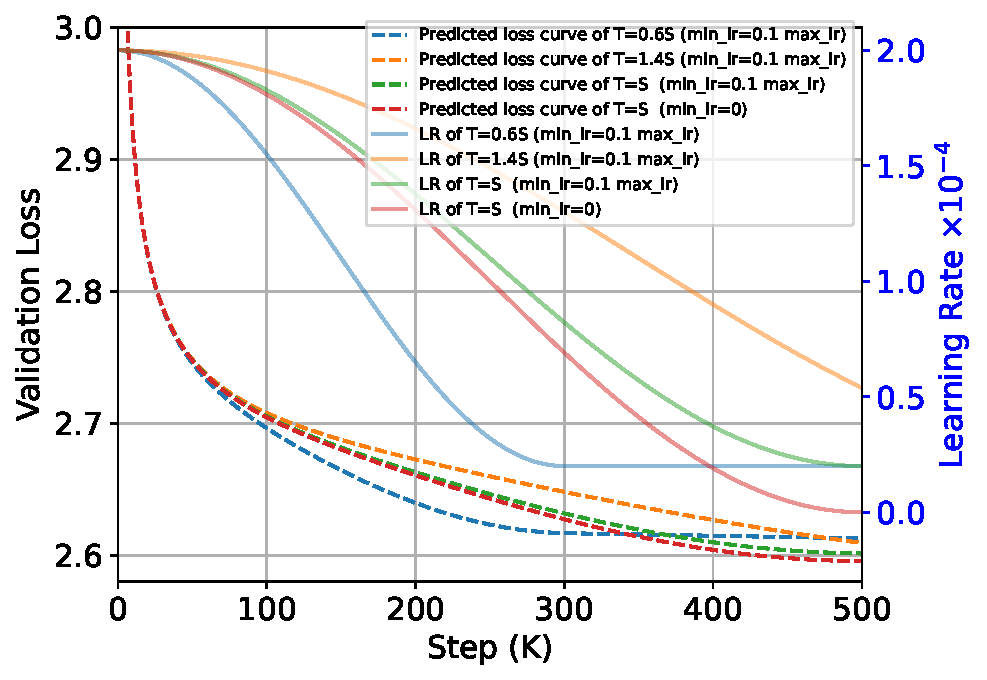
\includegraphics[width=\linewidth]{images/draw_phe/3-2-new.pdf}
    \caption{Predicted loss curves of different cycle length $T$ and min LR in cosine LRS. The results well align with previous studies.}
\label{fig:phe-cosine}
\vspace{-10pt}
\end{wrapfigure}



\subsection{\color{cyan} Determining cosine cycle length and minimum LR in cosine LRS.}
\vspace{-5pt}
Many papers have found that in LLM pre-training using cosine LRS, setting the cosine cycle length $T$ as the total steps $S$, and setting min LR as nearly 0 (rather than 10\% max LR) can lead to the optimal loss~\citep{hoffmann2022training,hu2024minicpm,hägele2024scaling,parmar2024reuse}. 
% Actually, the settings above have been a factual standard in LLM pre-training using cosine LRS.
We theoretically validate this observation using our equation in Fig.~\ref{fig:phe-cosine}. The predicted loss curve with $T=S$ and a minimum LR of 0 indeed achieves the optimal loss in the final step.
Moreover, our equation gives a quite intuitive explanation: setting $T>S$ leads to incomplete annealing, while $T<S$ leads to a small forward area $S_1$ due to early annealing. Thus, the optimal configuration is to set $T$ equal to $S$. Also, setting the minimum LR to $0$ maximizes the annealing amount, thereby increasing the annealing area $S_2$, which facilitates lower final loss.

\subsection{\color{cyan} It verifies and explains why WSD and multi-step cosine LRS are better.}
\vspace{-5pt}
\begin{figure}[ht]
    \centering
    \begin{subfigure}[b]{0.48\textwidth}
        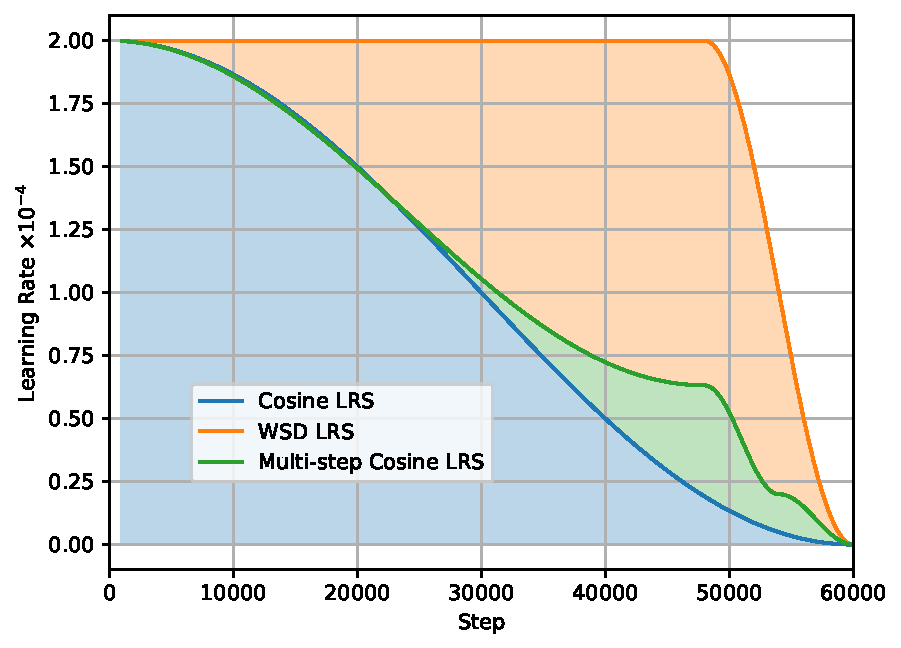
\includegraphics[width=\textwidth]{images/draw_phe/2.pdf}
        \caption{Learning rate curves of three types of LRS.}
    \end{subfigure}
    \hfill
    \begin{subfigure}[b]{0.48\textwidth}
        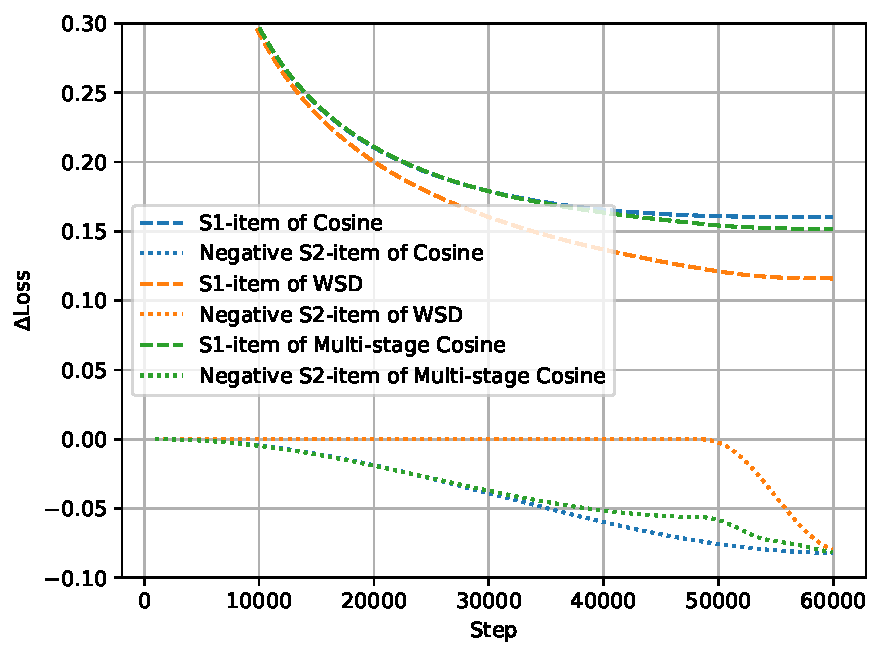
\includegraphics[width=\textwidth]{images/draw_phe/2-2.pdf}
        \caption{$S_1$-item and negative $S_2$-item of different LRS.}
    \end{subfigure}
    \caption{The comparison between $S_1$-item and negative $S_2$-item in different LRS.}
\label{fig:phe-match}
\end{figure}

Recent studies have shown that WSD LRS~\citep{hu2024minicpm} and multi-step cosine LRS~\citep{deepseek-ai2024deepseek} result in lower loss compared to the traditional cosine LRS. 
%Our experiments also support this finding (refer to the ground-truth loss in Fig.~\ref{fig:prediction-cosine},~\ref{fig:prediction-multi-cosine},~\ref{fig:prediction-wsd}). 
We validate and elucidate this finding using our proposed equation. Fig.~\ref{fig:phe-match} shows the learning rate curve (left) and the predicted loss drop (right) for different LRS.
The results suggest that for WSD and multi-step cosine LRS, the negative $S_2$-item ($-C\cdot S_2$) is slightly larger than that of the cosine LRS, whereas the $S_1$-item ($A\cdot S_1^{-\alpha}$) is significantly lower.
Specifically, both the WSD LRS and multi-step cosine LRS unintentionally employ strategies that marginally reduces $S_2$ but substantially increases $S_1$, leading to an overall decrease in validation loss.


\subsection{\color{cyan} Determining Optimal Annealing Ratio of WSD Scheduler.}
\vspace{-5pt}
In the case of WSD LRS, it is crucial to ascertain the optimal annealing ratio for training steps. 
~\citet{hägele2024scaling} found that there is an optimal annealing ratio for WSD LRS, and both excessively high or low annealing ratios lead to sub-optimal model performance. 
This phenomenon can be further elucidated through our proposed equation. 
Specifically, a high annealing ratio results in a significant reduction of the forward area $S_1$ while a low annealing ratio leads a diminished annealing area $S_2$. 
Our scaling law equation describes the trade-off between the forward area $S_1$ and the annealing area $S_2$ about the annealing ratio.

Fig.~\ref{fig:phe-match:1} depicts the final loss predicted by our equation for various annealing ratios and total training steps. 
The predictions form parabola-like curves, and align well with the actual experimental results reported in previous studies.
This suggests that a moderate annealing ratio, typically around 10\% to 20\%, is optimal, as it balances $S_1$ and $S_2$ to maximize their combined effect, thereby minimizing the overall validation loss.
Moreover, our equation can directly predict the optimal annealing ratio for different total steps without large-scale experiments, which saves a lot of resources. 

\begin{figure}[tbp]
    \centering
    \begin{subfigure}[b]{0.48\textwidth}
        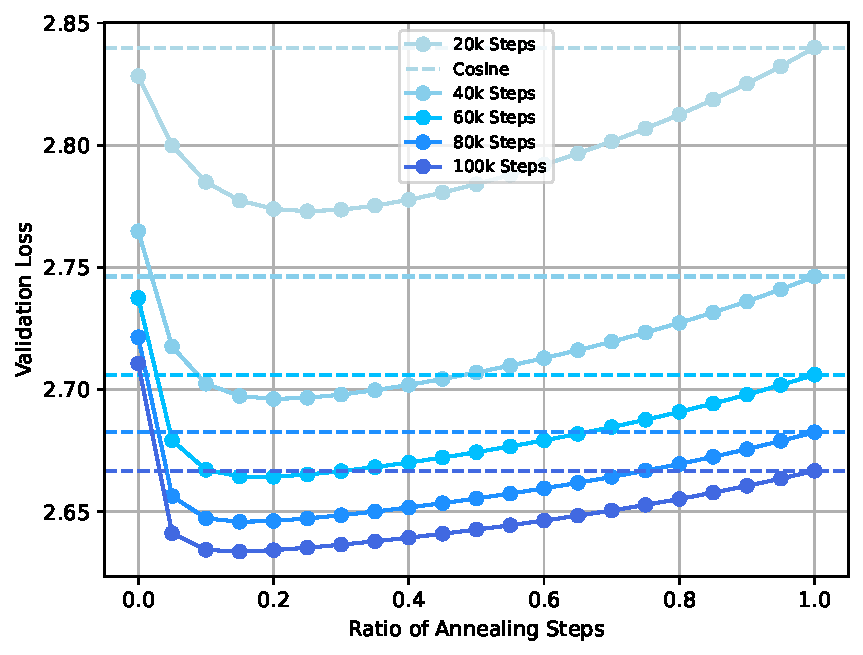
\includegraphics[width=\textwidth]{images/wsd_ratio.pdf}
        \caption{The relationship between the predicted final loss and the ratio of annealing steps under the condition of different total steps.}
    \end{subfigure}
    \hfill
    \begin{subfigure}[b]{0.48\textwidth}
        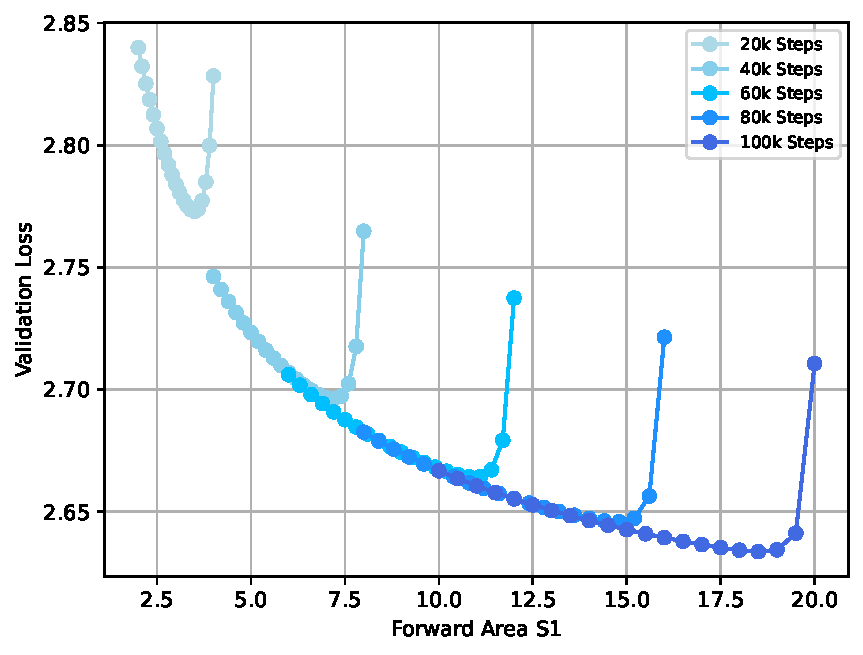
\includegraphics[width=\textwidth]{images/s1_loss.pdf}
        \caption{The relationship between predicted final loss and the forward area $S_1$ of different total steps. Different points denote different annealing ratios.}
    \end{subfigure}
    \caption{Illustration of the predicted loss in relation to the ratio of annealing steps and the forward area in WSD LRS (cosine annealing), presenting parabola-like curves, with a distinct optimal loss.}
\label{fig:phe-match:1}
\vspace{-10pt}
\end{figure}

\vspace{-5pt}
\subsection{\color{cyan} Many other takeaways} 
\vspace{-5pt}
Moreover, we use our equation to verify and explain more phenomena as follows:
\textbf{(1) }Appendix~\ref{apx:takeaway-sharpdrop}: why loss drops more sharply when LR anneals, aligned with previous works~\citep{loshchilov2016sgdr,simple-scalable-cpt2024,deepseek-ai2024deepseek}.
\textbf{(2)} Appendix~\ref{apx:takeaway-constant-cosine}: the comparison between constant and cosine LRS, aligned with previous works~\citep{hu2024minicpm}.
\textbf{(3)} Appendix~\ref{apx:takeaway-anneal-func}: how to choose the optimal annealing function in WSD LRS, aligned with previous works~\citep{hägele2024scaling}.
\textbf{(4)} Appendix~\ref{apx:takeaway-cpt-peaklr} and~\ref{apx:takeaway-cpt-step}: how to re-warmup (including re-warmup peak LR and steps) in continual pre-training, aligned with previous works~\citep{gupta2023continualpretraininglargelanguage}.
Given the instances above, we believe that our equation can help analyze and select more training recipes in specific scenarios.
